Diversas técnicas e algoritmos são utilizadas nas aplicações de reconhecimento automático de placas de carros. Neste capítulo é feito um aprofundamento teórico sobre as técnicas utilizadas em todas as etapas do desenvolvimento do trabalho, explicando os principais algoritmos e conceitos aplicados na construção da ferramenta.

\section{Processamento de Imagens}
\label{sec:processamentoimagens}

Lorem ipsum dolor sit amet, consectetur adipiscing elit, sed do eiusmod tempor incididunt ut labore et dolore magna aliqua. Ut enim ad minim veniam, quis nostrud exercitation ullamco laboris nisi ut aliquip ex ea commodo consequat. Duis aute irure dolor in reprehenderit in voluptate velit esse cillum dolore eu fugiat nulla pariatur. Excepteur sint occaecat cupidatat non proident, sunt in culpa qui officia deserunt mollit anim id est laborum

\section{Reconhecimento Ótico de Caracteres}
\label{sec:ocr}

Reconhecimento Ótico de Caracteres (\emph{Optical Character Recognition}, OCR)
consiste da conversão de textos em formato de imagem para o formato reconhecido
por máquina. É o método mais eficiente para fazer o processamento de imagem para
texto de acordo com Mohit et al.~\cite{mohit2015designing}.

Uma ferramenta conhecida de OCR é o
\emph{Tesseract}\footnote{https://github.com/tesseract-ocr/tesseract}. É uma ferramenta
\emph{open source} de reconhecimento ótico de caracteres que suporta múltiplas
línguas.  É essencialmente um algoritmo de comparação de \emph{templates}, e as
amostras de caracteres podem ser auto-treinadas.~\cite{ho2016intelligent}

Neste trabalho, implementaremos um \emph{software} de reconhecimento ótico de caracteres focado especificamente em reconhecer caracteres de placas de transito brasileiras utilizando aprendizado de máquina com o algoritmo \emph{K-Nearest Neighbors} que será fundamentado na seção ~\ref{sec:knearest}

\section{Filtro Bilateral}
\label{sec:bilateralfilter}

Lorem ipsum dolor sit amet, consectetur adipiscing elit, sed do eiusmod tempor incididunt ut labore et dolore magna aliqua. Ut enim ad minim veniam, quis nostrud exercitation ullamco laboris nisi ut aliquip ex ea commodo consequat. Duis aute irure dolor in reprehenderit in voluptate velit esse cillum dolore eu fugiat nulla pariatur. Excepteur sint occaecat cupidatat non proident, sunt in culpa qui officia deserunt mollit anim id est laborum

\section{Detecção de Bordas}
\label{sec:detecbordas}

Detecção de bordas é um método de processamento de imagem desenvolvido para detectar pixels de borda. os pixels de borda são pixels em que a intensidade da imagem muda abruptamente, e as bordas são conjuntos de pixels de borda conexos.\cite{gonzalez1977digital}

\subsection{Filtro de Sobel}
\label{sec:sobel}

Lorem ipsum dolor sit amet, consectetur adipiscing elit, sed do eiusmod tempor incididunt ut labore et dolore magna aliqua. Ut enim ad minim veniam, quis nostrud exercitation ullamco laboris nisi ut aliquip ex ea commodo consequat. Duis aute irure dolor in reprehenderit in voluptate velit esse cillum dolore eu fugiat nulla pariatur. Excepteur sint occaecat cupidatat non proident, sunt in culpa qui officia deserunt mollit anim id est laborum

\section{Limiarização}
\label{sec:limiarizacao}

Lorem ipsum dolor sit amet, consectetur adipiscing elit, sed do eiusmod tempor incididunt ut labore et dolore magna aliqua. Ut enim ad minim veniam, quis nostrud exercitation ullamco laboris nisi ut aliquip ex ea commodo consequat. Duis aute irure dolor in reprehenderit in voluptate velit esse cillum dolore eu fugiat nulla pariatur. Excepteur sint occaecat cupidatat non proident, sunt in culpa qui officia deserunt mollit anim id est laborum

\subsection{Método de Otsu}
\label{sec:otsu}

Lorem ipsum dolor sit amet, consectetur adipiscing elit, sed do eiusmod tempor incididunt ut labore et dolore magna aliqua. Ut enim ad minim veniam, quis nostrud exercitation ullamco laboris nisi ut aliquip ex ea commodo consequat. Duis aute irure dolor in reprehenderit in voluptate velit esse cillum dolore eu fugiat nulla pariatur. Excepteur sint occaecat cupidatat non proident, sunt in culpa qui officia deserunt mollit anim id est laborum

\section{Operações Morfológicas}
\label{sec:morfologicas}

Lorem ipsum dolor sit amet, consectetur adipiscing elit, sed do eiusmod tempor incididunt ut labore et dolore magna aliqua. Ut enim ad minim veniam, quis nostrud exercitation ullamco laboris nisi ut aliquip ex ea commodo consequat. Duis aute irure dolor in reprehenderit in voluptate velit esse cillum dolore eu fugiat nulla pariatur. Excepteur sint occaecat cupidatat non proident, sunt in culpa qui officia deserunt mollit anim id est laborum

\subsection{Erosão}
\label{sec:erosao}

Lorem ipsum dolor sit amet, consectetur adipiscing elit, sed do eiusmod tempor incididunt ut labore et dolore magna aliqua. Ut enim ad minim veniam, quis nostrud exercitation ullamco laboris nisi ut aliquip ex ea commodo consequat. Duis aute irure dolor in reprehenderit in voluptate velit esse cillum dolore eu fugiat nulla pariatur. Excepteur sint occaecat cupidatat non proident, sunt in culpa qui officia deserunt mollit anim id est laborum

\subsection{Dilatação}
\label{sec:dilatacao}

Lorem ipsum dolor sit amet, consectetur adipiscing elit, sed do eiusmod tempor incididunt ut labore et dolore magna aliqua. Ut enim ad minim veniam, quis nostrud exercitation ullamco laboris nisi ut aliquip ex ea commodo consequat. Duis aute irure dolor in reprehenderit in voluptate velit esse cillum dolore eu fugiat nulla pariatur. Excepteur sint occaecat cupidatat non proident, sunt in culpa qui officia deserunt mollit anim id est laborum

\subsection{Abertura}
\label{sec:abertura}

Lorem ipsum dolor sit amet, consectetur adipiscing elit, sed do eiusmod tempor incididunt ut labore et dolore magna aliqua. Ut enim ad minim veniam, quis nostrud exercitation ullamco laboris nisi ut aliquip ex ea commodo consequat. Duis aute irure dolor in reprehenderit in voluptate velit esse cillum dolore eu fugiat nulla pariatur. Excepteur sint occaecat cupidatat non proident, sunt in culpa qui officia deserunt mollit anim id est laborum

\subsection{Fechamento}
\label{sec:fechamento}

Lorem ipsum dolor sit amet, consectetur adipiscing elit, sed do eiusmod tempor incididunt ut labore et dolore magna aliqua. Ut enim ad minim veniam, quis nostrud exercitation ullamco laboris nisi ut aliquip ex ea commodo consequat. Duis aute irure dolor in reprehenderit in voluptate velit esse cillum dolore eu fugiat nulla pariatur. Excepteur sint occaecat cupidatat non proident, sunt in culpa qui officia deserunt mollit anim id est laborum

\section{K-Nearest Neighbors}
\label{sec:knearest}

\emph{K-Nearest Neighbors} é um dos mais simples algoritmos de classificação disponíveis para aprendizado supervisionado em aprendizado de máquina.~\cite{opencv2014knearest} Aprendizado supervisionado é tarefa de inferir uma função a partir de dados de treinamento rotulados. O algoritmo recebe um conjunto de exemplos como dados de treinamento e faz predições para os pontos não vistos com base nestes dados.~\cite{mohri2012foundations} A ideia do algoritmo \emph{K-Nearest Neighbors} é encontrar a combinação mais próxima de um determinado dado de teste em um espaço de dados.~\cite{opencv2014knearest}

\begin{figure}[H]
	\centering
	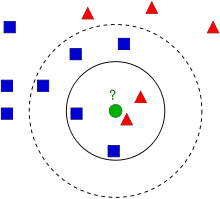
\includegraphics[width=50mm]{knn_theory.png}
	\caption{Exemplo de aplicação do K-Nearest Neighbors}
Fonte: Understanding k-Nearest Neighbour~\cite{opencv2014knearest}
	\label{fig:knearest_example}
\end{figure}

Em um caso hipotético de aplicação do algoritmo existem duas classes, a classe dos quadrados azuis e a classe dos triângulos vermelhos. Este exemplo está ilustrado na figura \ref{fig:knearest_example}. Pontos representando estas classes são espalhados em um espaço chamado de \emph{feature space}. Estes espaços são os espaços onde todos os dados estão projetados. Em um espaço de duas dimensões, como no exemplo, cada dado tem duas características, x e y. Em um espaço de três dimensões, cada dado teria 3 característica, em N dimensões, N características.

Na adição de um novo dado no \emph{feature space}, ele deve ser classificado como uma das duas classes. Este é o chamado de processo de classificação, onde o algoritmo é aplicado.

Um método é o de calcular quem é o vizinho mais próximo. Na imagem, este seria o triangulo vermelho. Este método é chamado de \emph{Nearest Neighbor}, ou o vizinho mais próximo, pois a classificação só depende de um vizinho.

Outro método seria checar múltiplos vizinhos para ver quantos vizinhos de cada classe o novo dado possui. Na imagem, o triangulo vermelho é o vizinho mais próximo, mas, considerando múltiplos vizinhos, é possível classificar o novo dado na classe dos quadrados azuis, pois existem mais vizinhos desta classe. Este método é chamado de \emph{k Nearest Neighbors}, pois ele considera uma quantidade pré determinada \emph{k} de vizinhos para classificar seus novos dados. ~\cite{opencv2014knearest}

Neste projeto o algoritmo \emph{K-Nearest Neighbors} é utilizado na implementação do reconhecedor ótico de caracteres encontrados em placas de transito brasileiras. São utilizados como dados de teste as letras maiúsculas e números na fonte \emph{Mandatory}, e são aproximados os valores dos caracteres segmentados da placa com base nestes. Como teremos apenas um valor para cada classe, cada classe representando um caractere diferente, utilizaremos apenas o vizinho mais próximo para classificar nossos caracteres. Tendo um conjunto de treinamento maior, é possível aumentar este valor.
 